\chapter{Results}
\epigraph{``Another quote.''}{\vspace{10pt}Another author}
\label{chapter:results}
\newpage

This chapter presents the results obtained while evaluating the proposed algorithm/mechanisms. The discussion and analysis of results are presented in the \nameref{chapter:discussion} chapter.


\section{Performance Evaluation}

\subsection{Calibration Results}

Figures \ref{fig:mcd_evolution_history}, \ref{fig:ts_evolution_history}, and \ref{fig:lmcd_evolution_history} show the evolution of the Pearson correlation coefficient ($R$) for each \acrshort{uq} method across generations and population members during \acrshort{cmaes} optimization. Each line represents a different population member, the shaded area indicates the range of $R$ values across the population at each generation, and the color encodes the value of the hyperparameter being optimized.

\begin{figure}[htbp]
    \centering
    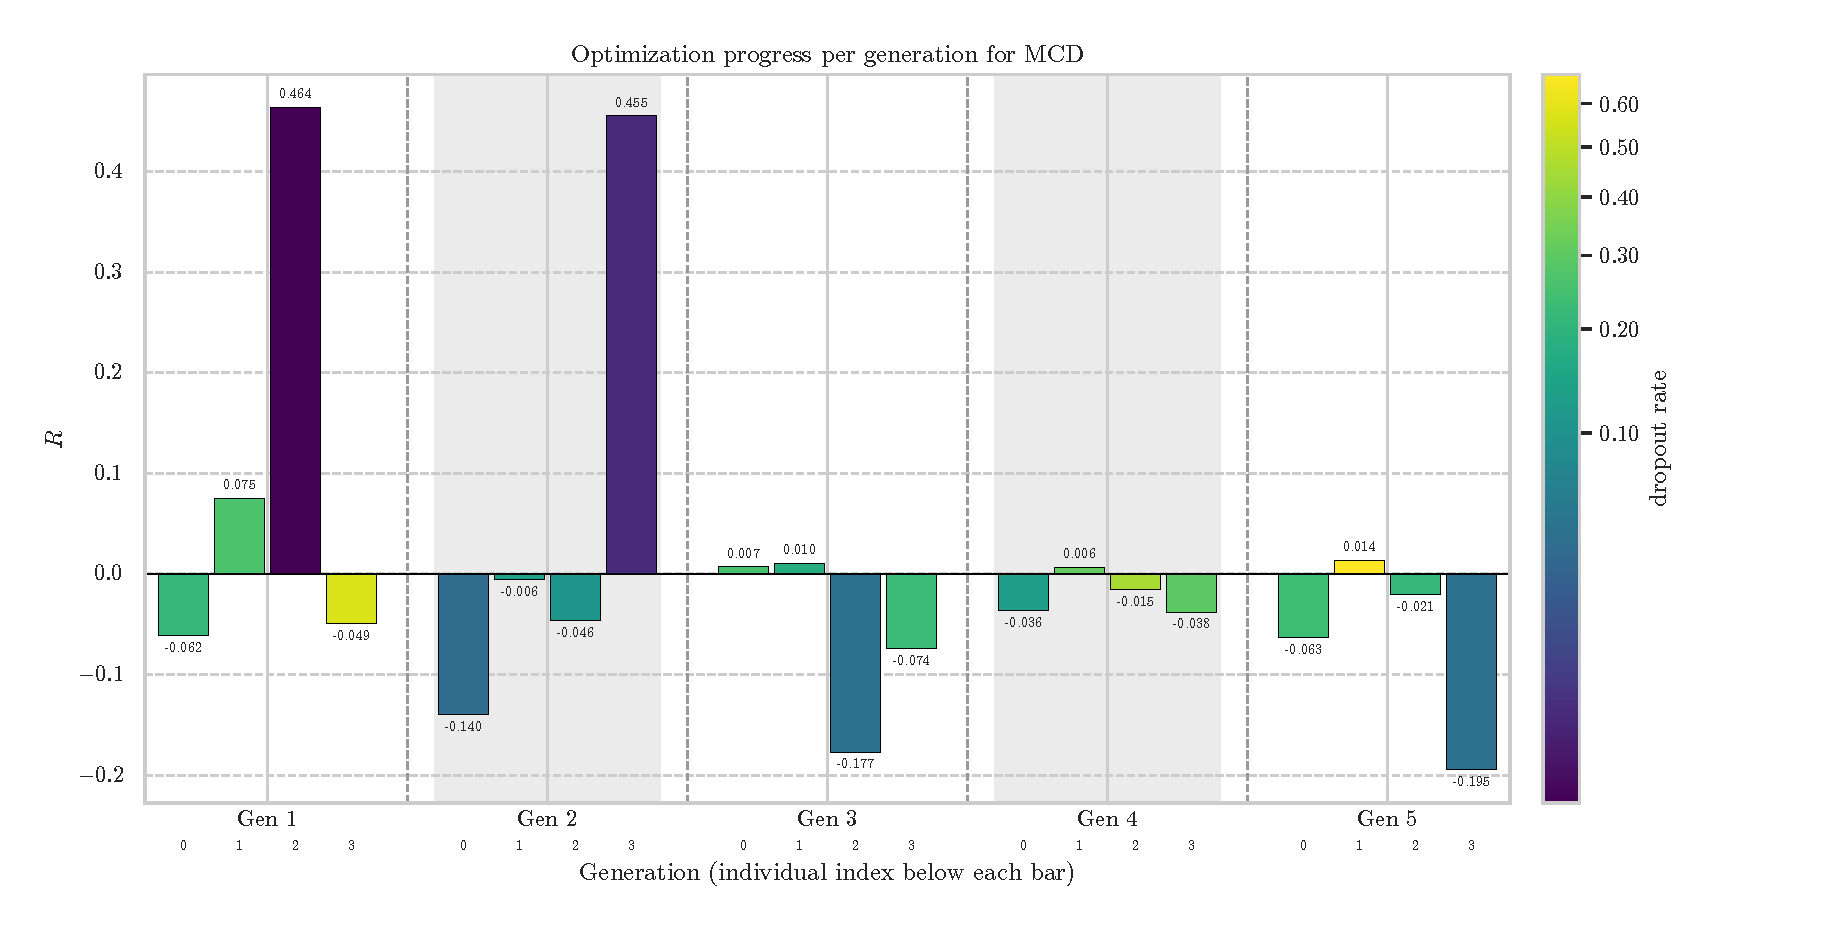
\includegraphics[width=0.9\linewidth]{../images/mcd_evolution_history.eps}
    \caption{Evolution history of the correlation coefficient ($R$) for the \acrshort{mcd} method.}
    \label{fig:mcd_evolution_history}
\end{figure}

The \acrshort{mcd} evolution in Figure \ref{fig:mcd_evolution_history} shows that the method is quite sensitive to hyperparameter tuning; the best performance on the calibration dataset is achieved with dropout rates $< 0.01$, beyond which performance drops sharply and the variance across the population increases dramatically. This suggests an unstable optimization landscape and a very narrow optimal range, which can be a problem for tuning this method in practice. The best performance is achieved with a dropout rate of $\mcdRate$ and a mean $R$ of $\mcdCalibrationR$ across folds. This rate is much lower than the commonly used $0.1$ or $0.2$ and is consistent with the findings of \cite{rodriguez2024uncertainty}.

\begin{figure}[htbp]
    \centering
    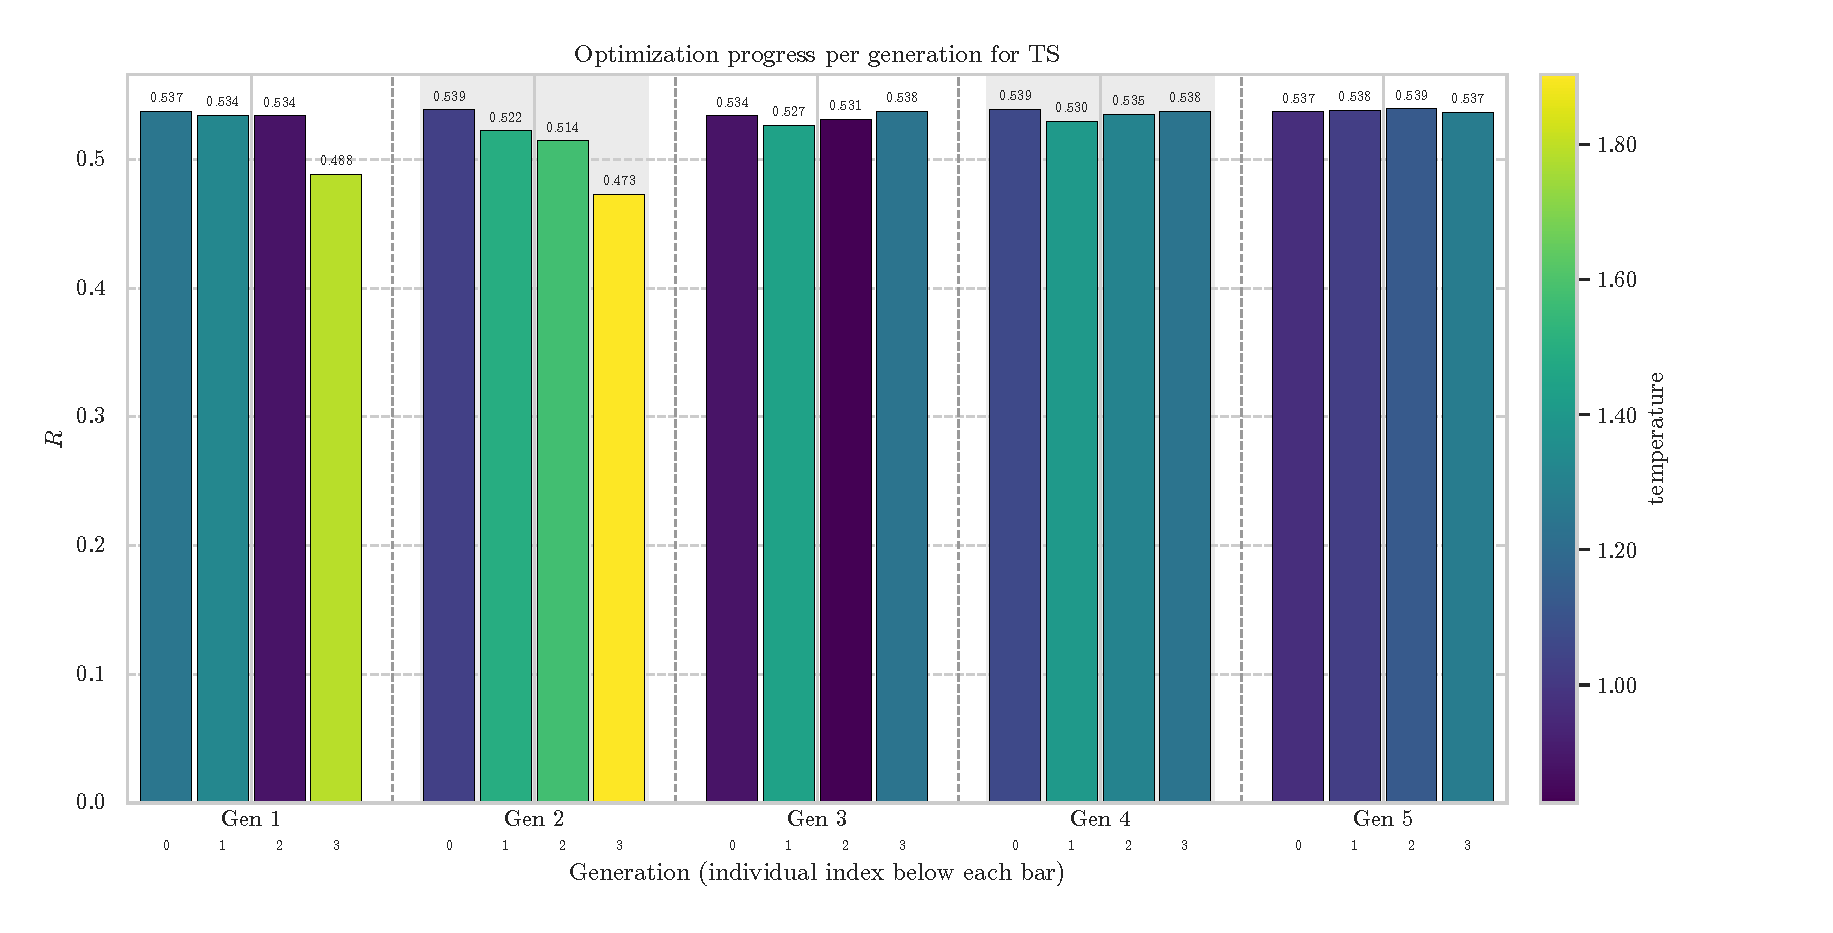
\includegraphics[width=0.9\linewidth]{../images/ts_evolution_history.eps}
    \caption{Evolution history of the correlation coefficient ($R$) for the \acrshort{ts} method.}
    \label{fig:ts_evolution_history}
\end{figure}

In contrast, Figure \ref{fig:ts_evolution_history} shows that \acrshort{ts} provides consistent uncertainty estimates across a wide range of temperature values, with the best performance achieved around $\tau = \tsTemp$ and a mean $R$ of $\tsCalibrationR$ across folds. Even at the sampled extremes, performance varies less than for the dropout-based methods, suggesting that \acrshort{ts} is less sensitive to hyperparameter selection in this experiment and may be a practical choice when computational resources for tuning are limited.

\begin{figure}[htbp]
    \centering
    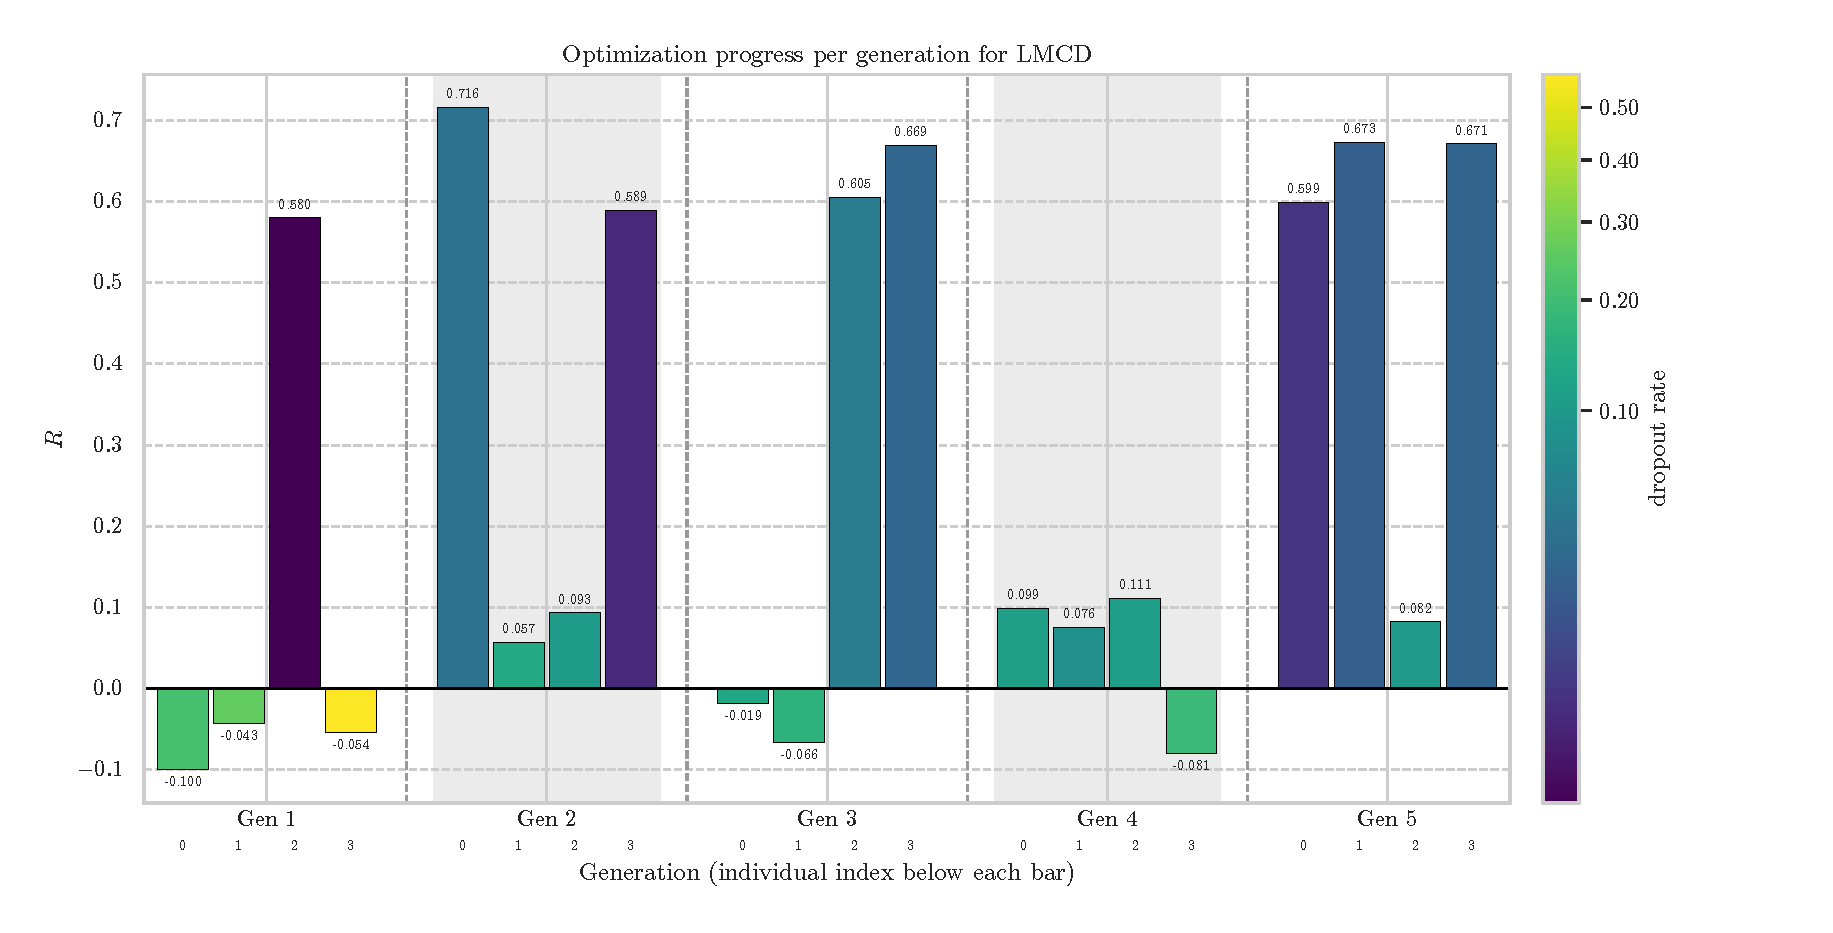
\includegraphics[width=0.9\linewidth]{../images/lmcd_evolution_history.eps}
    \caption{Evolution history of the correlation coefficient ($R$) for the \acrshort{lmcd} method.}
    \label{fig:lmcd_evolution_history}
\end{figure}

Figure \ref{fig:lmcd_evolution_history} shows that \acrshort{lmcd} follows a pattern similar to \acrshort{mcd}, where lower dropout ranges provide the best performance, but it remains more stable across a wider range of values. The best performance is achieved with a dropout rate of $\lmcdRate$ and a mean $R$ of $\lmcdCalibrationR$ across folds. \acrshort{lmcd} thus supports the trend of lower dropout rates yielding better performance, although its optimum is an order of magnitude higher than that of \acrshort{mcd}, which indicates that \acrshort{lmcd} is more robust to changes in the dropout rate and therefore easier and cheaper to tune.

\begin{figure}[htbp]
    \centering
    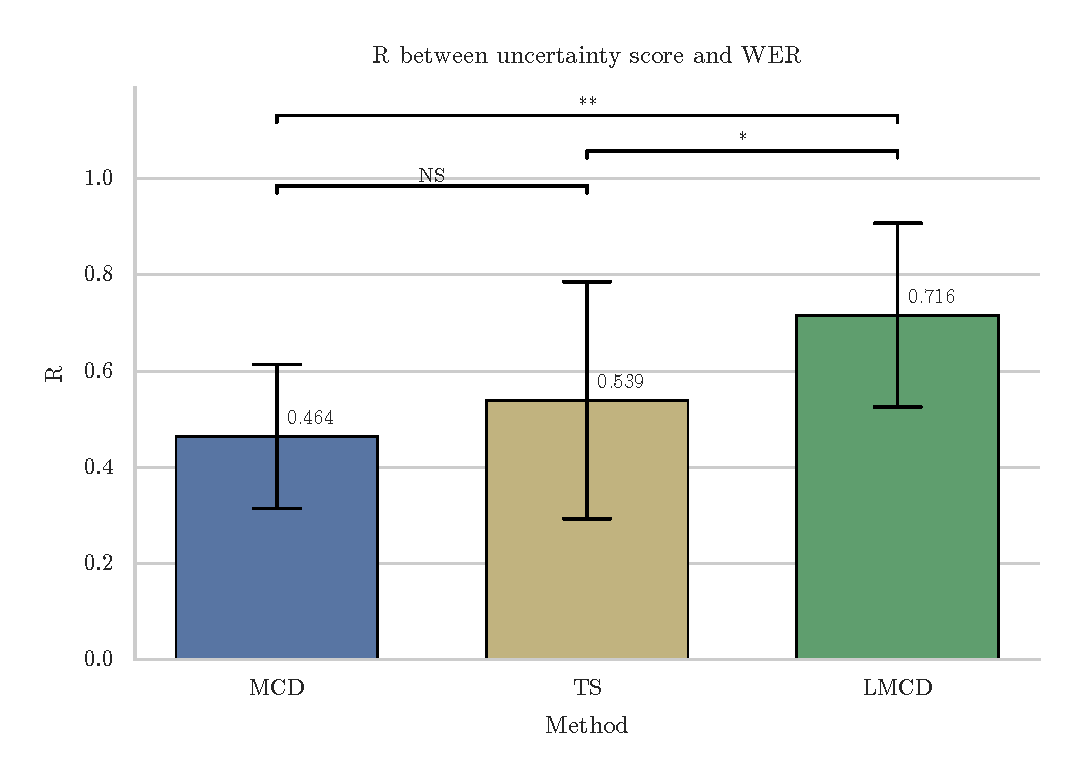
\includegraphics[width=0.9\linewidth]{../images/best_calibration.eps}
    \caption{Best calibration results for each \acrshort{uq} method. The whiskers represent the standard deviation of the $R$ values across folds.}
    \label{fig:best_calibration_results}
\end{figure}

Figure \ref{fig:best_calibration_results} summarizes the best calibration results for each method.

\subsection{Test Results}

Having selected the best hyperparameters on the calibration split, we evaluate them on the held-out test split. Figure \ref{fig:best_test_results} summarizes the best test results for each method, and the per-method values are collected in Table \ref{tab:summary}.

\begin{figure}[htbp]
    \centering
    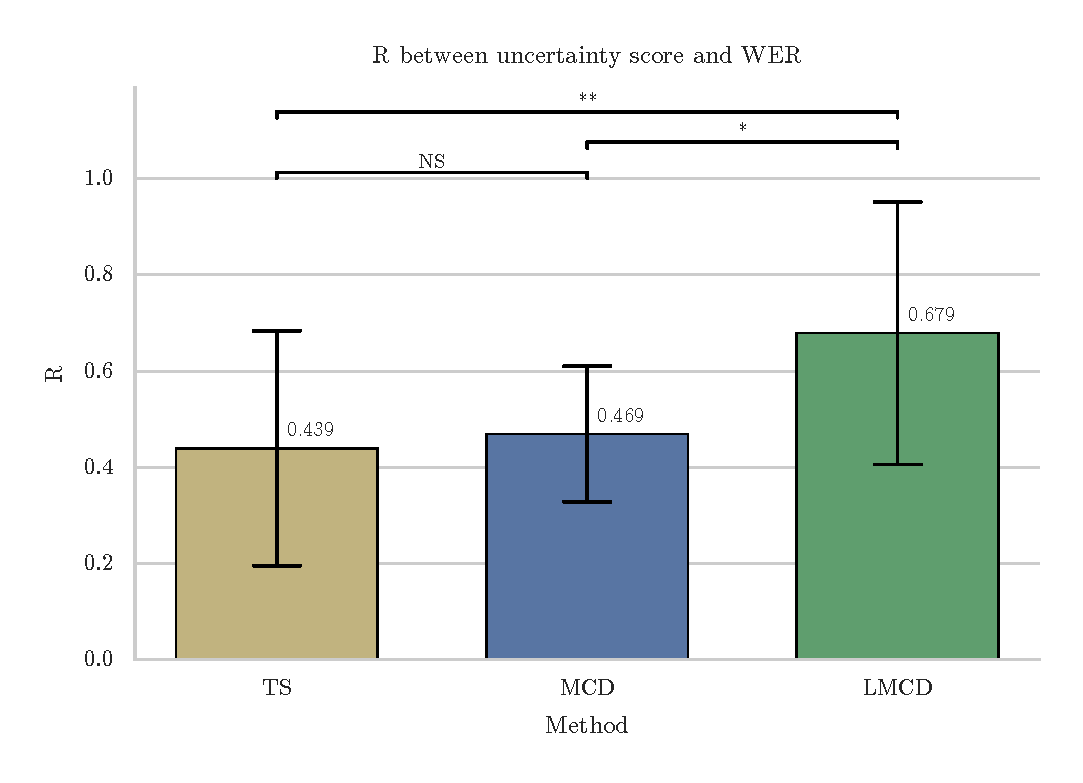
\includegraphics[width=0.9\linewidth]{../images/best_test.eps}
    \caption{Best test results for each \acrshort{uq} method. The whiskers represent the standard deviation of the $R$ values across folds.}
    \label{fig:best_test_results}
\end{figure}

\section{Statistical Tool Assumptions Tests}
\todo{aplicar normalidad y homocedasticidad tests a los $R$ values para justificar el uso de un t-test, o decidir usar un test no paramétrico.}

The statistical tool used is the Wilcoxon signed-rank test, a non-parametric test that operates on the ranks of the paired differences and therefore does not assume that the $R$ values are normally distributed. Because no normality or homoscedasticity assumption is required, there are no distributional assumptions to verify before applying it; the only requirements are that the observations be paired across folds and measured on at least an ordinal scale, both of which hold by construction since every method is evaluated on the same ten folds.

\section{Statistical Tool Results}

\subsection{Validity}

Table \ref{tab:wilcoxon_single_calibration} reports a one-sided Wilcoxon signed-rank test of whether each method's median $R$ is greater than zero across the ten folds, at $\alpha = 0.05$. All three methods reject the null hypothesis at $p = 0.0009766$, the smallest value attainable with $N = 10$, which corresponds to every fold yielding a positive correlation. This establishes that each method produces uncertainty scores that are consistently and positively correlated with the \acrshort{wer}, but it does not by itself rank the methods.

\begin{table}[ht]
    \centering
    \begin{tabular}{|l|l|l|l|l|}
        \hline
        Method          & N  & Median & p-value   & Verdict     \\ \hline
        \acrshort{mcd}  & 10 & 0.5068 & 0.0009766 & Significant \\ \hline
        \acrshort{ts}   & 10 & 0.6634 & 0.0009766 & Significant \\ \hline
        \acrshort{lmcd} & 10 & 0.7965 & 0.0009766 & Significant \\ \hline
    \end{tabular}
    \caption{Wilcoxon signed-rank validity test on the calibration dataset.}
    \label{tab:wilcoxon_single_calibration}
\end{table}

Table \ref{tab:wilcoxon_single_test} repeats the one-sided validity evaluation on the held-out test split. The null hypothesis is again rejected for every method ($p \leq 0.001953$), confirming that the positive correlation between uncertainty and \acrshort{wer} persists on data that was not used for hyperparameter selection.

\begin{table}[ht]
    \centering
    \begin{tabular}{|l|l|l|l|l|}
        \hline
        Method          & N  & Median & p-value   & Verdict     \\ \hline
        \acrshort{mcd}  & 10 & 0.4658 & 0.0009766 & Significant \\ \hline
        \acrshort{ts}   & 10 & 0.4262 & 0.001953  & Significant \\ \hline
        \acrshort{lmcd} & 10 & 0.7888 & 0.001953  & Significant \\ \hline
    \end{tabular}
    \caption{Wilcoxon signed-rank validity test on the test dataset.}
    \label{tab:wilcoxon_single_test}
\end{table}

\subsection{Pairwise Comparison}

Given that the validity test holds on both splits, we compare the methods with a paired, two-sided Wilcoxon signed-rank test at $\alpha = 0.05$. Table \ref{tab:wilcoxon_pairwise} reports the pairwise p-values on both splits. On the calibration split, \acrshort{lmcd} differs significantly from both \acrshort{mcd} ($p = 0.0020$) and \acrshort{ts} ($p = 0.027$), whereas \acrshort{mcd} and \acrshort{ts} are statistically indistinguishable ($p = 0.084$). The same ranking carries over to the held-out test split, where \acrshort{lmcd} remains significantly distinct from both \acrshort{mcd} ($p = 0.020$) and \acrshort{ts} ($p = 0.0059$), while \acrshort{mcd} and \acrshort{ts} stay indistinguishable ($p = 0.49$).

\begin{table}[ht]
    \centering
    \begin{tabular}{|l|l|l|}
        \hline
        Comparison                        & Calibration p-value & Test p-value \\ \hline
        \acrshort{lmcd} vs \acrshort{mcd} & 0.0020              & 0.020        \\ \hline
        \acrshort{lmcd} vs \acrshort{ts}  & 0.027               & 0.0059       \\ \hline
        \acrshort{mcd} vs \acrshort{ts}   & 0.084               & 0.49         \\ \hline
    \end{tabular}
    \caption{Pairwise two-sided Wilcoxon signed-rank test p-values between methods on the calibration and test datasets.}
    \label{tab:wilcoxon_pairwise}
\end{table}

\section{Obtained Metrics}

Table \ref{tab:summary} collects the optimal hyperparameter and the mean Pearson correlation between the uncertainty score and the \acrshort{wer}, averaged across the ten folds, for each method on both splits. \acrshort{lmcd} attains the highest correlation on the test split ($\lmcdTestR$), ahead of \acrshort{mcd} ($\mcdTestR$) and \acrshort{ts} ($\tsTestR$), and stays close to its calibration value, whereas \acrshort{ts} degrades the most between calibration and test.

\begin{table}[ht]
    \centering
    \begin{tabular}{|l|c|c|c|}
        \hline
        Method          & Optimal hyperparameter & Calibration $R$   & Test $R$   \\ \hline
        \acrshort{ts}   & $\tau = \tsTemp$       & \tsCalibrationR   & \tsTestR   \\ \hline
        \acrshort{mcd}  & dropout $= \mcdRate$   & \mcdCalibrationR  & \mcdTestR  \\ \hline
        \acrshort{lmcd} & dropout $= \lmcdRate$  & \lmcdCalibrationR & \lmcdTestR \\ \hline
    \end{tabular}
    \caption{Optimal hyperparameter and mean Pearson correlation ($R$) between the uncertainty score and \acrshort{wer}, averaged across the ten folds, for each \acrshort{uq} method on the calibration and test splits.}
    \label{tab:summary}
\end{table}

Throughout this chapter each method is summarized by its mean $R$ across folds, whereas the validity tables report the median $R$ on which the Wilcoxon test operates; the mean falls below the median for every method because one fold consistently yields a markedly lower, and for some methods slightly negative, correlation that pulls the average down.
\newpage
